\documentclass[oneside]{pacotes/Ifba_tcc}

% 

% ======================================================


%======================================================
% PACKAGES
% ======================================================
\sloppy
\usepackage{color}
\usepackage{xcolor}
\usepackage{listings}
\usepackage{titlesec}
\usepackage{longtable}
\usepackage{tabularx}
\usepackage{booktabs}
\usepackage[table]{xcolor}
\usepackage[
  backend=biber,
  style=numeric,
  sorting=none
]{biblatex}

\addbibresource{02-elementos-textuais/12-referencias.bib}

% 
% ======================================================




% ======================================================
% PROLOG LISTINGS
% ======================================================

\lstdefinelanguage{SQL}{
    keywords={SELECT, INSERT, INTO, VALUES, CREATE, TABLE, PRIMARY, KEY, INT, VARCHAR},
    sensitive=false,
    comment=[l]{--},
    morestring=[b]'
}

\lstset{
    language=SQL,
    basicstyle=\ttfamily\small,
    keywordstyle=\bfseries,
    numbers=left,
    numberstyle=\tiny,
    frame=single,
    breaklines=true
}

% ======================================================
% PRE-TEXTUAL
% ======================================================
%=========================================================================
%DADOS DA INSTITUIÇÃO
\logoInst{
\includegraphics[width=0.4
\textwidth]{./03-figuras/logo_engenharia}}

%======================================================================================================
%DADOS DO TRABALHO
%************************************************************************************
\titulo{Engenharia Clínica e Gestão de Ativos}

\subtitulo{Monitorização de inventário, manutenção preventiva e calibração de dispositivos
médicos}

\autor{
Beatriz Ribeiro A107272\\
Clara Carvalho A107195\\
Dinis Rosa A107159\\
Renata Bravo A107246
}


%DADOS DA INSTITUIÇÃO
%****************************************************************************************************
\instituicao{Universidade do Minho} 
\curso{Licenciatura em Engenharia Biomédica} 
\local{UC de Base de Dados} 
\data{2025/2026} 
%========================================================================================================

% ======================================================
% DOCUMENT
% ======================================================
\begin{document}

\pretextual
\frenchspacing
\imprimircapa
\input{./01/indice}

\textual
\chapter{ Introdução}
\section{ Contextualização}
Na sua definição mais básica, uma base de dados é um conjunto de informações inter-relacionadas, utilizadas para armazenar e organizar dados de forma a facilitar a sua gestão e o acesso. Os dados referem-se a qualquer informação capturada sobre uma entidade e os seus atributos. À medida que uma coleção de dados cresce e assume maior complexidade, torna-se mais difícil manter a organização e a acessibilidade, surgindo a base de dados como a solução central para facilitar a interpretação desta informação.

Neste âmbito, os Sistemas de Base de Dados permitem-nos armazenar, recuperar e relacionar dados de forma estruturada. A plataforma MySQL, um dos sistemas mais utilizados, serve como interface de gestão para bases de dados relacionais através da linguagem SQL. No setor da saúde, estas ferramentas são fulcrais para garantir o funcionamento eficiente das instituições, nomeadamente na gestão de dispositivos médicos. A monitorização e manutenção destes equipamentos, apoiadas por bases de dados, são essenciais para o controlo operacional diário, garantindo que a tecnologia médica é utilizada com a máxima eficiência.

A manutenção regular é fundamental para assegurar a segurança dos pacientes e a qualidade dos serviços de saúde. Equipamentos em condições subótimas podem levar a diagnósticos incorretos ou tratamentos inadequados, colocando vidas em risco. Dada a complexidade dos aparelhos hospitalares, é imprescindível um sistema organizado que facilite o agendamento de manutenções preventivas e corretivas. Um sistema bem estruturado permite antecipar falhas, minimizar interrupções e garantir que os aparelhos cumpram as normas de segurança. Além disso, a rastreabilidade dos históricos permite identificar tendências de desgaste, otimizando recursos e reduzindo custos com reparos emergenciais ou substituições prematuras, promovendo, em última análise, a sustentabilidade operacional e financeira do hospital.

\newpage
\section{ Apresentação do Caso de Estudo}
O presente caso de estudo foca-se no desenvolvimento de um sistema para a gestão e acompanhamento da manutenção de equipamentos hospitalares. O sistema centraliza informações sobre os dispositivos, a sua localização geográfica nas unidades de saúde e os departamentos responsáveis.

A solução proposta integra os seguintes tópicos:

\begin{itemize}
    \item Gestão de Intervenções: Registo de ordens de serviço, históricos de manutenção e acompanhamento técnico.
\end{itemize}

\begin{itemize}
    \item Gestão de Recursos: Monitorização dos técnicos envolvidos, inventário de peças utilizadas e relação com fornecedores.
\end{itemize}

\begin{itemize}
    \item Controlo Financeiro: Rastreabilidade dos custos associados a cada intervenção e análise de desgaste dos ativos ao longo do tempo.
\end{itemize}

\section{ Motivação e Objetivos}
A motivação deste trabalho reside na aplicação prática dos conceitos de planeamento e desenvolvimento de bases de dados relacionais a um cenário real e complexo. O objetivo central é projetar uma solução que garanta a integridade e a acessibilidade dos dados hospitalares.

Para alcançar este propósito, o projeto divide-se nos seguintes objetivos específicos:

\begin{itemize}
    \item Modelação: Elaboração dos modelos conceptual (Diagrama Entidade-Associação), lógico e físico.
\end{itemize}

\begin{itemize}
    \item Implementação: Criação da base de dados em MySQL e respetivo povoamento com dados realistas.
\end{itemize}

\begin{itemize}
    \item Programação SQL: Desenvolvimento de subprogramas avançados, incluindo procedimentos (procedures), funções e triggers, para automatizar tarefas e facilitar a extração de métricas relevantes para a gestão hospitalar.
\end{itemize}
\chapter{ Modelo Conceptual}


Um modelo conceptual consiste numa representação gráfica que permite visualizar as ligações entre diferentes conceitos e ideias. Este tipo de modelo é desenvolvido a partir da análise de uma base de dados, na qual a informação é organizada em entidades, atributos e chaves primárias, sendo também definidos os respetivos relacionamentos entre esses elementos. 
Numa fase inicial, é fundamental identificar as entidades a analisar, bem como os seus atributos, estabelecendo também as relações entre elas, de modo a representar de forma coerente a lógica do mundo real.

Na notação de Chen, as entidades são representadas por retângulos verdes, os atributos por elipses de cor roxa e as relações entre entidades por losangos amarelos inseridos em retângulos verdes. Os atributos-chave destacam-se por estarem sublinhados e a negrito.

Para definir corretamente as relações, a cardinalidade assume um papel essencial, pois indica quantas ocorrências de uma entidade podem estar associadas a outra. As relações podem ser classificadas em três tipos: um para um (1:1), um para muitos (1:N) e muitos para muitos (N:N). Este último ocorre quando uma entidade pode associar-se a várias ocorrências de outra entidade e vice-versa, originando normalmente uma entidade associativa.

Relativamente às ligações entre entidades, uma linha simples indica que a participação na relação é opcional, enquanto uma linha dupla representa uma participação obrigatória.
A fig. 1 apresenta um diagrama Entidade-Relacionamento (ER), criado com recurso ao \textit{software} TerraER.

\begin{figure}[h]
    \centering
    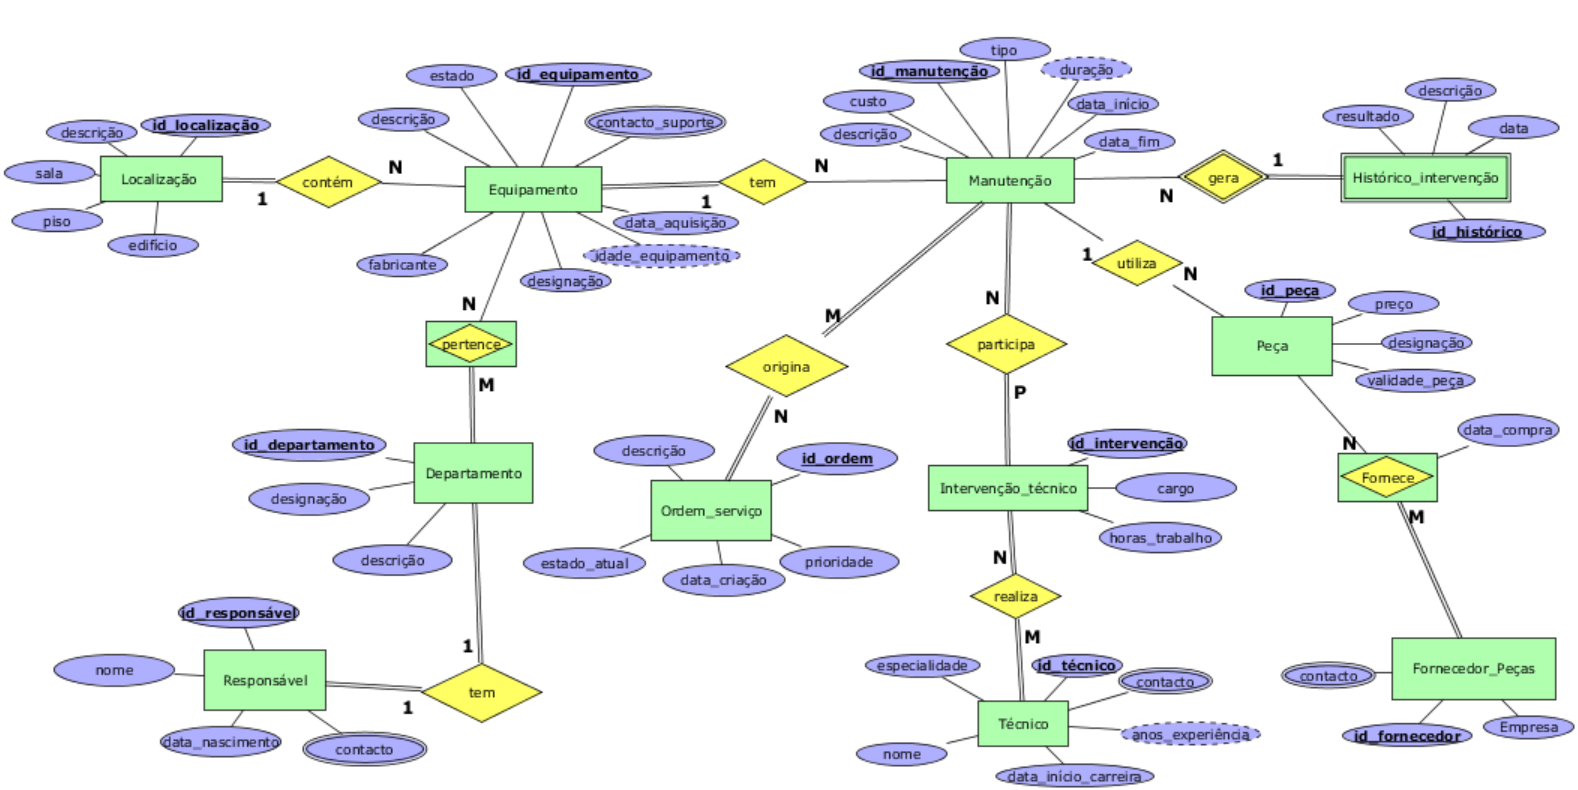
\includegraphics[width=1\textwidth]{./03-figuras/modelo_conceptual}
    \caption{Modelo Conceptual.}
\end{figure}


\section{ Entidades}
Entidades são objetos ou conceitos representados no banco de dados.  
Neste modelo, definiram-se as seguintes entidades:

\begin{itemize}
    \item \textbf{Localização}: Armazena informações sobre os locais onde os equipamentos se encontram;
    \item \textbf{Equipamento}: Contém os dados relativos aos equipamentos existentes;
    \item \textbf{Manutenção}: Regista informações sobre as manutenções realizadas nos equipamentos;
    \item \textbf{Histórico\_intervenção}: Guarda o histórico das intervenções efetuadas;
    \item \textbf{Peça}: Armazena dados sobre as peças utilizadas nas manutenções;
    \item \textbf{Fornecedor\_peças}: Contém informações sobre os fornecedores de peças;
    \item \textbf{Técnico}: Regista os dados dos técnicos responsáveis pelas intervenções;
    \item \textbf{Intervenção\_técnico}: Representa a participação dos técnicos nas intervenções;
    \item \textbf{Ordem\_serviço}: Guarda informações sobre as ordens de serviço criadas;
    \item \textbf{Departamento}: Contém os dados dos departamentos da organização;
    \item \textbf{Responsável}: Armazena informações sobre os responsáveis associados aos departamentos.
\end{itemize}


\section{ Atributos}
Atributos são características ou propriedades que descrevem uma entidade. Cada atributo tem
um tipo de dado associado, que define o tipo de valor que o atributo pode armazenar, como números
inteiros, texto, datas, entre outros.

De seguida, apresentam-se os atributos associados a cada uma das entidades.

\textbf{Localização:}
\begin{itemize}
    \item id\_localização - Identificador único da localização
    \item descrição - Descrição da localização
    \item sala - Sala onde se encontra o equipamento
    \item piso - Piso da localização
    \item edifício - Edifício correspondente
\end{itemize}

\textbf{Equipamento:}
\begin{itemize}
    \item id\_equipamento - Identificador único do equipamento
    \item descrição - Descrição do equipamento
    \item estado - Estado atual do equipamento
    \item fabricante - Fabricante do equipamento
    \item designação - Nome/designação do equipamento
    \item data\_aquisição - Data de aquisição do equipamento
    \item idade\_equipamento - Idade do equipamento
    \item contacto\_suporte - Contacto de suporte técnico
\end{itemize}

\textbf{Manutenção:}
\begin{itemize}
    \item id\_manutenção - Identificador único da manutenção
    \item tipo - Tipo de manutenção
    \item duração - Duração da manutenção
    \item data\_inicio - Data de início da manutenção
    \item data\_fim - Data de fim da manutenção
    \item custo - Custo da manutenção
    \item descrição - Descrição da manutenção
\end{itemize}

\textbf{Histórico\_Intervenção:}
\begin{itemize}
    \item id\_histórico - Identificador único do histórico
    \item descrição - Descrição da intervenção
    \item resultado - Resultado da intervenção
    \item data - Data da intervenção
\end{itemize}

\textbf{Peça:}
\begin{itemize}
    \item id\_peça - Identificador único da peça
    \item designação - Nome/designação da peça
    \item preço - Preço da peça
    \item validade\_peça - Validade da peça
\end{itemize}

\textbf{Fornecedor\_peças:}
\begin{itemize}
    \item id\_fornecedor - Identificador único do fornecedor
    \item empresa - Nome da empresa fornecedora
    \item contacto - Contacto do fornecedor
\end{itemize}

\textbf{Técnico:}
\begin{itemize}
    \item id\_técnico - Identificador único do técnico
    \item nome - Nome do técnico
    \item especialidade - Especialidade do técnico
    \item contacto - Contacto do técnico
    \item anos\_experiência - Anos de experiência
    \item data\_inicio\_carreira - Data de início de carreira
\end{itemize}

\textbf{Intervenção\_técnico:}
\begin{itemize}
    \item id\_intervenção - Identificador único da intervenção
    \item cargo - Função do técnico na intervenção
    \item horas\_trabalho - Número de horas trabalhadas
\end{itemize}

\textbf{Ordem\_serviço:}
\begin{itemize}
    \item id\_ordem - Identificador único da ordem de serviço
    \item descrição - Descrição da ordem
    \item estado\_atual - Estado atual da ordem
    \item data\_criação - Data de criação da ordem
    \item prioridade - Prioridade da ordem
\end{itemize}

\textbf{Departamento:}
\begin{itemize}
    \item id\_departamento - Identificador único do departamento
    \item designação - Nome/designação do departamento
    \item descrição - Descrição do departamento
\end{itemize}

\textbf{Responsável:}
\begin{itemize}
    \item id\_responsável - Identificador único do responsável
    \item nome - Nome do responsável
    \item data\_nascimento - Data de nascimento
    \item contacto - Contacto do responsável
\end{itemize}
\chapter{ Modelo Lógico}
\par O modelo lógico de uma base de dados representa a fase de transição entre a abstração do modelo conceptual e a implementação técnica no Sistema de Gestão de Base de Dados (SGBD). Nesta etapa, os conceitos e ideias definidos anteriormente são convertidos num modelo representacional, onde as entidades dão lugar a tabelas e os atributos tornam-se colunas com tipos de dados específicos.
\par Ao contrário do modelo conceptual, o modelo lógico foca-se na eficiência da estrutura de dados e nas relações formais. Através de processos de normalização, procura-se obter um conjunto de tabelas que minimizem a redundância e assegurem a integridade referencial, permitindo um registo de dados robusto e coerente com a lógica do mundo real. \\

\begin{figure}[h]
    \centering
    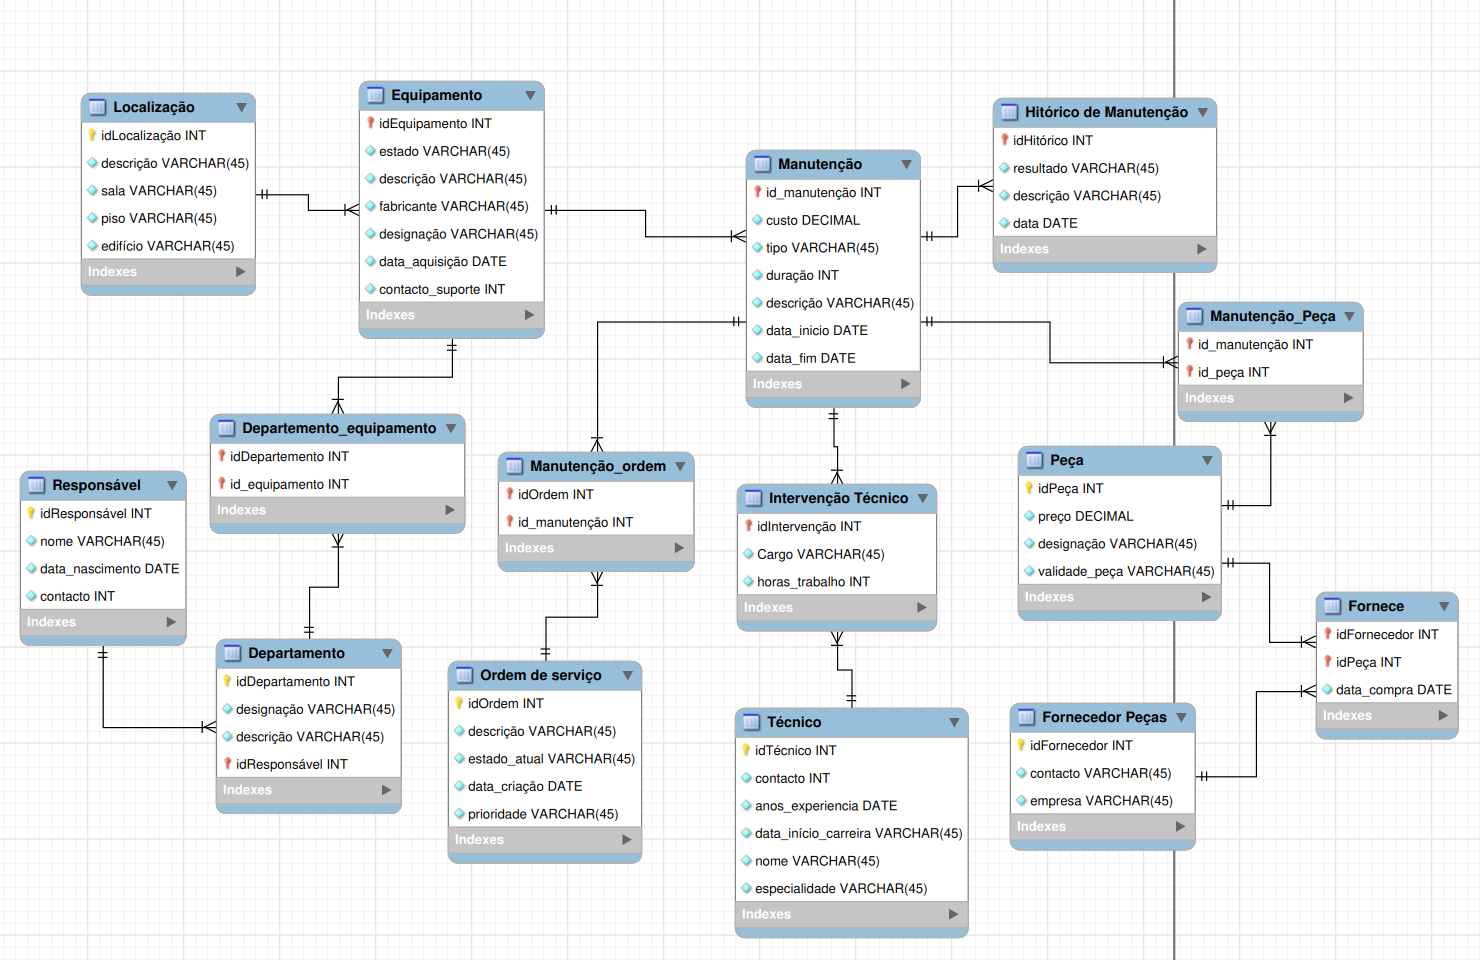
\includegraphics[width=1.05\textwidth]{./03-figuras/modelo_logico}
    \caption{Modelo lógico.}
\end{figure}
\input{02-texto/4-modelo_fisico}
\chapter{ Documentação de atributos}

Na tabela apresentada abaixo, é possível observar uma caracterização detalhada de cada atributo pertencente às diferentes entidades do modelo.

Destaca-se a coluna “Tipos de dados e tamanho”, que indica o tipo de dado associado a cada atributo, como número inteiro (INT), data (DATE) ou texto (VARCHAR), bem como o respetivo tamanho quando aplicável.

Para além disso, assumem especial importância as colunas de chave primária e chave estrangeira. A chave primária corresponde ao atributo (ou conjunto de atributos) que identifica de forma única cada registo numa tabela (por exemplo, \textit{id\_equipamento} na entidade EQUIPAMENTO ou \textit{id\_manutenção} na entidade MANUTENÇÃO).

Por outro lado, as chaves estrangeiras são responsáveis por estabelecer ligações entre tabelas distintas, referenciando chaves primárias de outras entidades (por exemplo, uma manutenção está associada a um equipamento através de uma chave estrangeira).

Estas chaves são fundamentais na organização de uma base de dados relacional, garantindo a integridade dos dados e facilitando a sua consulta e manipulação.

\renewcommand{\arraystretch}{1.0}
\rowcolors{2}{gray!10}{white}

{\tiny
\begin{longtable}{p{2.5cm} p{3cm} p{5cm} p{2cm} c}
\toprule
\textbf{Entidade} & \textbf{Atributo} & \textbf{Descrição} & \textbf{Tipo} & \textbf{Nulo} \\
\midrule
\endfirsthead

\toprule
\textbf{Entidade} & \textbf{Atributo} & \textbf{Descrição} & \textbf{Tipo} & \textbf{Nulo} \\
\midrule
\endhead

\multicolumn{5}{l}{\textbf{Localização}} \\
\midrule
 & id_localizacao & Identificador da localização & INT & Não \\
 & descricao & Descrição da localização & VARCHAR(100) & Não \\
 & sala & Sala & VARCHAR(3) & Não \\
 & piso & Piso & VARCHAR(2) & Não \\
 & edificio & Edifício & VARCHAR(2) & Não \\

\midrule
\multicolumn{5}{l}{\textbf{Equipamento}} \\
\midrule
 & id_equipamento & Identificador do equipamento & INT & Não \\
 & descricao & Descrição do equipamento & VARCHAR(100) & Não \\
 & estado & Estado do equipamento & VARCHAR(50) & Não \\
 & fabricante & Fabricante & VARCHAR(100) & Não \\
 & designacao & Designação & VARCHAR(100) & Não \\
 & data_aquisicao & Data de aquisição & DATE & Não \\
 & idade_equipamento & Idade do equipamento & INT & Não \\
 & contacto_suporte & Contacto de suporte & VARCHAR(20) & Sim \\
 & id_localizacao & Localização associada & INT & Não \\
 & id_departamento & Departamento associado & INT & Não \\

\midrule
\multicolumn{5}{l}{\textbf{Manutenção}} \\
\midrule
 & id_manutencao & Identificador da manutenção & INT & Não \\
 & tipo & Tipo de manutenção & VARCHAR(50) & Não \\
 & duracao & Duração & INT & Não \\
 & data_inicio & Data de início & DATE & Não \\
 & data_fim & Data de fim & DATE & Não \\
 & custo & Custo & DECIMAL & Não \\
 & descricao & Descrição & VARCHAR(200) & Não \\
 & id_equipamento & Equipamento associado & INT & Não \\

\midrule
\multicolumn{5}{l}{\textbf{Histórico_intervenção}} \\
\midrule
 & id_historico & Identificador do histórico & INT & Não \\
 & descricao & Descrição & VARCHAR(200) & Não \\
 & resultado & Resultado & VARCHAR(100) & Não \\
 & data & Data & DATE & Não \\
 & id_manutencao & Manutenção associada & INT & Não \\

\midrule
\multicolumn{5}{l}{\textbf{Peça}} \\
\midrule
 & id_peca & Identificador da peça & INT & Não \\
 & designacao & Designação & VARCHAR(100) & Não \\
 & preco & Preço & DECIMAL & Não \\
 & validade_peca & Validade & DATE & Não \\

\midrule
\multicolumn{5}{l}{\textbf{Fornecedor_peças}} \\
\midrule
 & id_fornecedor & Identificador do fornecedor & INT & Não \\
 & empresa & Nome da empresa & VARCHAR(100) & Não \\
 & contacto & Contacto & VARCHAR(10) & Não \\

\midrule
\multicolumn{5}{l}{\textbf{Técnico}} \\
\midrule
 & id_tecnico & Identificador do técnico & INT & Não \\
 & nome & Nome & VARCHAR(100) & Não \\
 & especialidade & Especialidade & VARCHAR(100) & Não \\
 & contacto & Contacto & VARCHAR(10) & Não \\
 & anos_experiencia & Anos de experiência & INT & Não \\
 & data_inicio_carreira & Data início carreira & DATE & Não \\

\midrule
\multicolumn{5}{l}{\textbf{Intervenção_técnico}} \\
\midrule
 & id_intervencao & Identificador da intervenção & INT & Não \\
 & cargo & Cargo na intervenção & VARCHAR(50) & Não \\
 & horas_trabalho & Horas de trabalho & INT & Não \\
 & id_tecnico & Técnico associado & INT & Não \\
 & id_manutencao & Manutenção associada & INT & Não \\

\midrule
\multicolumn{5}{l}{\textbf{Ordem_serviço}} \\
\midrule
 & id_ordem & Identificador da ordem & INT & Não \\
 & descricao & Descrição & VARCHAR(200) & Não \\
 & estado_atual & Estado atual & VARCHAR(50) & Não \\
 & data_criacao & Data de criação & DATE & Não \\
 & prioridade & Prioridade & VARCHAR(20) & Não \\

\midrule
\multicolumn{5}{l}{\textbf{Departamento}} \\
\midrule
 & id_departamento & Identificador do departamento & INT & Não \\
 & designacao & Designação & VARCHAR(100) & Não \\
 & descricao & Descrição & VARCHAR(200) & Não \\

\midrule
\multicolumn{5}{l}{\textbf{Responsável}} \\
\midrule
 & id_responsavel & Identificador do responsável & INT & Não \\
 & nome & Nome & VARCHAR(100) & Não \\
 & data_nascimento & Data nascimento & DATE & Não \\
 & contacto & Contacto & VARCHAR(20) & Não \\
 & id_departamento & Departamento associado & INT & Não \\

\bottomrule
\end{longtable}
}




\chapter{ Povoamento}

\section{Povoamento da entidade “Localização”}
{\small
\begin{lstlisting}{SQL}
INSERT INTO Localização (id_ocalização, descrição, sala, piso, edifício) VALUES
(1, 'Sala de Servidores Principal', '101', '1', '1'),
(2, 'Laboratório de Informática', '202', '2', '2'),
(3, 'Armazém de Equipamentos', '001', '0', '3'),
(4, 'Sala de Reuniões Norte', '301', '3', '1'),
(5, 'Centro de Controlo', '100', '1', '4'),
(6, 'Oficina de Manutenção', '050', '0', '2'),
(7, 'Sala de Comunicações', '205', '2', '1'),
(8, 'Depósito Técnico', '010', '0', '3'),
(9, 'Sala de Monitorização', '401', '4', '4'),
(10, 'Receção Principal', '001', '0', '1');
\end{lstlisting}
}

\section{Povoamento da entidade “Equipamento”}
{\small
\begin{lstlisting}[breaklines]{SQL}
INSERT INTO Equipamento (idEquipamento, estado, descrição, fabricante, designação, data_aquisição, idade_equipamento, contacto_suporte) VALUES
(1, 'Operacional', 'Ventilador Pulmonar Avançado', 'Draeger', 'Evita V500', '2023-05-15', 2, '912345678'),
(2, 'Operacional', 'Ecógrafo Portátil 4D', 'GE Healthcare', 'Vivid iq', '2022-11-20', 3, '922334455'),
(3, 'Em Manutenção', 'Monitor de Sinais Vitais', 'Philips', 'IntelliVue MX450', '2024-01-10', 2, '933445566'),
(4, 'Operacional', 'Desfibrilhador Automático', 'Zoll', 'R Series', '2023-08-05', 2, '966778899'),
(5, 'Avariado', 'Bomba de Infusão Contínua', 'B. Braun', 'Infusomat P', '2021-03-30', 5, '911223344'),
(6, 'Operacional', 'Eletrocardiógrafo 12 Canais', 'Mortara', 'ELI 250', '2022-06-12', 3, '922887766'),
(7, 'Operacional', 'Aspirador de Secreções Hospitalar', 'Medela', 'Dominant Flex', '2023-12-01', 2, '933554433'),
(8, 'Em Manutenção', 'Oximetro de Pulso de Mesa', 'Masimo', 'Rad-97', '2024-02-15', 2, '911001122'),
(9, 'Operacional', 'Termómetro de Infravermelhos Pro', 'Welch Allyn', 'CareTemp', '2024-03-01', 2, '966009988'),
(10, 'Operacional', 'Esfigmomanómetro Digital', 'Omron', 'HBP-1320', '2023-09-20', 2, '911998877');
\end{lstlisting}
}

\section{Povoamento da entidade “Departamento”}
{\small
\begin{lstlisting}[breaklines]{SQL}
INSERT INTO Departamento (id_departamento, designação, descrição, id_responsável) VALUES
(1, 'Cardiologia', 'Unidade de cuidados e diagnósticos cardíacos', 1),
(2, 'Imagiologia', 'Serviço de exames radiológicos e ecografias', 4),
(3, 'Urgências', 'Atendimento permanente de cuidados agudos', 2),
(4, 'Manutenção Técnica', 'Gestão de infraestruturas e biomédica', 3),
(5, 'Cuidados Intensivos', 'Unidade de monitorização crítica (UCI)', 5);
\end{lstlisting}
}

\section{Povoamento da entidade “Departamento Equipamento”}
{\small
\begin{lstlisting}[breaklines]{SQL}
INSERT INTO Departamento_equipamento (idDepartamento, id_equipamento) VALUES
(5, 1), 
(2, 2), 
(1, 3),  
(3, 4),  
(4, 8);
\end{lstlisting}
}

\section{Povoamento da entidade “Responsável”}
{\small
\begin{lstlisting}[breaklines]{SQL}
INSERT INTO Responsável (id_responsável, nome, data_nascimento, contacto) VALUES
(1, 'Dra. Ana Martins', '1975-03-12', '912345678'),
(2, 'Dr. Carlos Santos', '1982-07-25', '922334455'),
(3, 'Dr. Ricardo Pereira', '1980-11-05', '933445566'),
(4, 'Dra. Sofia Oliveira', '1988-01-30', '966778899'),
(5, 'Dr. Miguel Ferreira', '1970-05-18', '911223344');
\end{lstlisting}
}

\section{Povoamento da entidade “Ordem de Serviço”}
{\small
\begin{lstlisting}[breaklines]{SQL}
INSERT INTO Ordem de serviço (id_ordem, descrição, estado_atual, data_criação, prioridade) VALUES
(1, 'Verificação anual do ventilador pulmonar', 'Concluída', '2025-01-10', 'Alta'),
(2, 'Calibração do ecógrafo portátil', 'Concluída', '2025-02-05', 'Média'),
(3, 'Reparação do monitor de sinais vitais', 'Em Curso', '2025-03-01', 'Alta'),
(4, 'Substituição de bateria do desfibrilhador', 'Concluída', '2025-01-20', 'Alta'),
(5, 'Manutenção preventiva da bomba de infusão', 'Pendente', '2025-03-15', 'Média'),
(6, 'Revisão do eletrocardiógrafo', 'Concluída', '2025-02-18', 'Baixa'),
(7, 'Limpeza e teste do aspirador de secreções', 'Concluída', '2025-01-28', 'Baixa'),
(8, 'Diagnóstico do oxímetro de pulso', 'Em Curso', '2025-03-10', 'Alta'),
(9, 'Verificação do termómetro de infravermelhos', 'Concluída', '2025-02-25', 'Baixa'),
(10, 'Calibração do esfigmomanómetro digital', 'Pendente', '2025-03-20', 'Média');
\end{lstlisting}
}

\section{Povoamento da entidade “Manutenção”}
{\small
\begin{lstlisting}[breaklines]{SQL}
INSERT INTO Manutenção (id_manutenção, custo, tipo, duração, descrição, data_inicio, data_fim) VALUES
(1, 350.00, 'Preventiva', 4, 'Manutenção preventiva anual do ventilador', '2025-01-12', '2025-01-12'),
(2, 220.00, 'Calibração', 3, 'Calibração e ajuste do ecógrafo portátil', '2025-02-07', '2025-02-07'),
(3, 480.00, 'Corretiva', 8, 'Substituição de ecrã do monitor de sinais vitais', '2025-03-03', NULL),
(4, 150.00, 'Corretiva', 2, 'Substituição de bateria interna do desfibrilhador', '2025-01-22', '2025-01-22'),
(5, 310.00, 'Preventiva', 5, 'Revisão geral da bomba de infusão contínua', '2025-03-17', NULL),
(6, 180.00, 'Preventiva', 3, 'Revisão e limpeza do eletrocardiógrafo', '2025-02-20', '2025-02-20'),
(7, 90.00, 'Preventiva', 2, 'Limpeza e teste funcional do aspirador', '2025-01-29', '2025-01-29'),
(8, 260.00, 'Corretiva', 6, 'Diagnóstico e reparação do oxímetro de pulso', '2025-03-11', NULL),
(9, 70.00, 'Calibração', 1, 'Verificação de precisão do termómetro', '2025-02-26', '2025-02-26'),
(10, 120.00, 'Calibração', 2, 'Calibração do esfigmomanómetro digital', '2025-03-22', NULL);
\end{lstlisting}
}

\section{Povoamento da entidade “Manutenção Ordem”}
{\small
\begin{lstlisting}[breaklines]{SQL}
INSERT INTO Manutenção_ordem (idOrdem, id_manutenção) VALUES
(1, 1),
(2, 2),
(3, 3),
(4, 4),
(5, 5),
(6, 6),
(7, 7),
(8, 8),
(9, 9),
(10, 10);
\end{lstlisting}
}

\section{Povoamento da entidade “Histórico de Intervenção”}
{\small
\begin{lstlisting}[breaklines]{SQL}
INSERT INTO `Hitórico de Manutenção` (id_hitórico, resultado, descrição, data) VALUES
(1, 'Sucesso', 'Ventilador verificado e calibrado sem anomalias', '2025-01-12'),
(2, 'Sucesso', 'Ecógrafo calibrado, imagem dentro dos parâmetros', '2025-02-07'),
(3, 'Em Curso', 'Aguarda peça de substituição para o ecrã', '2025-03-03'),
(4, 'Sucesso', 'Bateria substituída, desfibrilhador operacional', '2025-01-22'),
(5, 'Em Curso', 'Revisão iniciada, bomba aguarda diagnóstico completo', '2025-03-17'),
(6, 'Sucesso', 'Eletrocardiógrafo revisto, traçado estável', '2025-02-20'),
(7, 'Sucesso', 'Aspirador limpo e testado, funcionamento normal', '2025-01-29'),
(8, 'Em Curso', 'Oxímetro em diagnóstico, sensor principal suspeito', '2025-03-11'),
(9, 'Sucesso', 'Termómetro verificado, desvio dentro da margem', '2025-02-26'),
(10, 'Pendente', 'Calibração agendada, equipamento operacional', '2025-03-22');
\end{lstlisting}
}

\section{Povoamento da entidade “Peça”}
{\small
\begin{lstlisting}[breaklines]{SQL}
INSERT INTO Peça (id_peça, preço, designação, validade_peça) VALUES
(1, 85.00, 'Filtro de ar HEPA ventilador', '2027-12-31'),
(2, 210.00, 'Sonda ecográfica convexa', '2028-06-30'),
(3, 320.00, 'Ecrã tátil monitor sinais vitais', '2029-01-01'),
(4, 95.00, 'Bateria Li-ion desfibrilhador', '2026-12-31'),
(5, 140.00, 'Rotor bomba de infusão', '2027-06-30'),
(6, 60.00, 'Cabo de eléctrodos ECG', '2028-01-01'),
(7, 45.00, 'Filtro aspirador secreções', '2027-03-31'),
(8, 175.00, 'Sensor SpO2 oxímetro de pulso', '2028-09-30'),
(9, 30.00, 'Pilhas alcalinas termómetro', '2026-06-30'),
(10, 55.00, 'Manguito esfigmomanómetro adulto', '2027-12-31');
\end{lstlisting}
}

\section{Povoamento da entidade “Fornece”}
{\small
\begin{lstlisting}[breaklines]{SQL}
INSERT INTO Fornece (id_fornecedor, id_peça, data_compra) VALUES
(1, 1, '2025-01-10'),  
(2, 2, '2025-02-05'),  
(3, 3, '2025-03-01'),  
(1, 4, '2025-01-20'), 
(4, 5, '2025-03-15'),  
(2, 6, '2025-02-18'),  
(5, 7, '2025-01-28'),  
(3, 8, '2025-03-10'), 
(5, 9, '2025-02-25'),  
(4, 10, '2025-03-20'); 
\end{lstlisting}
}

\section{Povoamento da entidade “Fornecedor Peças”}
{\small
\begin{lstlisting}[breaklines]{SQL}
INSERT INTO `Fornecedor Peças` (id_fornecedor, contacto, empresa) VALUES
(1, '210100200', 'MedTech Ibérica, Lda.'),
(2, '220200300', 'BioSupply Portugal, S.A.'),
(3, '230300400', 'HospitalTech, Lda.'),
(4, '240400500', 'ProMed Equipamentos, S.A.'),
(5, '250500600', 'ClinicalParts Europa, Lda.');
\end{lstlisting}
}

\section{Povoamento da entidade “Manutenção Peça”}
{\small
\begin{lstlisting}[breaklines]{SQL}
INSERT INTO Manutenção_Peça (id_manutenção, id_peça) VALUES
(1, 1), 
(2, 2),  
(3, 3),  
(4, 4), 
(5, 5), 
(6, 6), 
(7, 7),  
(8, 8), 
(9, 9),  
(10, 10);
\end{lstlisting}
}

\section{Povoamento da entidade “Técnico”}
{\small
\begin{lstlisting}[breaklines]{SQL}
INSERT INTO Técnico (id_técnico, contacto, anos_experiencia, data_inicio_carreira, nome, especialidade) VALUES
(1, '911222333', 9, '2015-01-15', 'Ricardo Pereira', 'Eletrónica Médica'),
(2, '922333444', 14, '2010-03-20', 'Marta Silveira', 'Imagiologia/Ressonância'),
(3, '933444555', 4, '2020-09-01', 'João Gouveia', 'Sistemas de Ventilação'),
(4, '966555666', 19, '2005-05-10', 'António Costa', 'Instrumentação Cirúrgica'),
(5, '911888999', 6, '2018-02-01', 'Beatriz Lopes', 'Monitorização Paramétrica');
\end{lstlisting}
}

\section{Povoamento da entidade “Intervenção Técnico”}
{\small
\begin{lstlisting}[breaklines]{SQL}
INSERT INTO Intervenção Técnico
(id_intervenção, cargo, horas_trabalho) VALUES
(1, 'Técnico Responsável', 4),
(2, 'Técnico Responsável', 3),
(3, 'Técnico Sénior', 8),
(4, 'Técnico Responsável', 2),
(5, 'Técnico Sénior', 5),
(6, 'Técnico Responsável', 3),
(7, 'Técnico Assistente', 2),
(8, 'Técnico Sénior', 6),
(9, 'Técnico Assistente', 1),
(10, 'Técnico Responsável', 2);

\end{lstlisting}
}

\input{02-texto/7-funcoes}
\input{02-texto/8-procedimentos}
\input{02-texto/9-triggers}
\input{02-texto/10-queries}
\input{02-texto/11-conclusao}
\input{02-texto/12-anexos}



 

\end{document}

% ======================================================
